% AVA Internal Report — LCO Key-Project Usage, Data Holdings and Sources
\documentclass[10pt,a4paper,oneside]{report}
\usepackage[T1]{fontenc}
\usepackage{tgtermes}
\usepackage{mathptmx}
\usepackage[a4paper,top=2.3cm,bottom=2.5cm,left=2.4cm,right=2.4cm,headsep=0.6cm]{geometry}
\usepackage{graphicx}
\usepackage{amsmath}
\usepackage{booktabs}
\usepackage{tabularx}
\usepackage{longtable}
\usepackage{xcolor}
\usepackage[hyphens]{url}
\usepackage[round,authoryear]{natbib}
\usepackage[font=small,labelfont=bf,labelsep=period,justification=justified,singlelinecheck=false]{caption}
\usepackage{titlesec}
\usepackage{fancyhdr}
\usepackage{tikz}
\usetikzlibrary{positioning,calc}
\usepackage[colorlinks=true,linkcolor={blue!60!black},citecolor={blue!60!black},urlcolor={blue!60!black}]{hyperref}
\PassOptionsToPackage{hyphens}{url}

%% AVA brand colours
\definecolor{avaInkBlue}{RGB}{26,58,92}
\definecolor{avaAbyss}{RGB}{10,22,40}
\definecolor{avaGold}{RGB}{212,160,23}
\definecolor{avaMidBlue}{RGB}{14,44,80}

\setlength{\parindent}{1.2em}
\setlength{\parskip}{0pt}
\setlength{\emergencystretch}{3em}
\renewcommand{\topfraction}{0.9}
\renewcommand{\textfraction}{0.08}
\renewcommand{\floatpagefraction}{0.75}
\setcounter{topnumber}{3}
\setcounter{totalnumber}{4}

\titleformat{\chapter}[block]{\normalfont\large\bfseries\color{avaInkBlue}}{\thechapter}{1em}{\MakeUppercase}
\titlespacing*{\chapter}{0pt}{0pt}{14pt}
\titleformat{\section}{\normalfont\normalsize\bfseries}{\thesection}{1em}{\MakeUppercase}
\titleformat{\subsection}{\normalfont\normalsize\bfseries}{\thesubsection}{1em}{}
\titleformat{\subsubsection}[runin]{\normalfont\normalsize\itshape}{\thesubsubsection}{0.6em}{}[.]
\titlespacing*{\section}{0pt}{12pt}{5pt}
\titlespacing*{\subsection}{0pt}{9pt}{3pt}

\pagestyle{fancy}
\fancyhf{}
\fancyhead[L]{\small\itshape\textcolor{avaInkBlue}{AGN Variability Archive}}
\fancyhead[R]{\small\itshape\textcolor{avaInkBlue}{LCO Usage Report}}
\fancyfoot[C]{\small\textcolor{avaInkBlue!60}{\thepage}}
\renewcommand{\headrulewidth}{0.4pt}
\renewcommand{\headrule}{\color{avaInkBlue!40}\hrule width\headwidth height\headrulewidth}
\fancypagestyle{plain}{\fancyhf{}\fancyfoot[C]{\small\textcolor{avaInkBlue!60}{\thepage}}\renewcommand{\headrulewidth}{0pt}}

\newcommand{\lcodb}{\texttt{lcodb}}
\makeatletter\newcommand{\inputtable}[1]{\@@input #1 }\makeatother

\graphicspath{{figures/}}
% generated by scripts/make_report.py -- do not edit
\newcommand{\avaMissing}{SDSS-RM201, SDSS-RM562, RX J22198-0935, PKS 0558-504, NGC 2617, IGR J17062-6143}
\newcommand{\expImagesH}{12,616}
\newcommand{\expImagesMs}{45.4}
\newcommand{\expSpectraH}{2,199}
\newcommand{\expSpectraMs}{7.92}
\newcommand{\firstImage}{2014-08-04}
\newcommand{\firstSpectrum}{2014-05-05}
\newcommand{\fracArcBlock}{95.0}
\newcommand{\fracFlatBlock}{96.1}
\newcommand{\fracImagesHdr}{0}
\newcommand{\fracSameSlit}{30}
\newcommand{\fracSixArcsec}{64}
\newcommand{\fracSkyPlaceholder}{100}
\newcommand{\gbpOneM}{336}
\newcommand{\gbpPerUsd}{0.746}
\newcommand{\gbpTotal}{9.0}
\newcommand{\gbpTotalHigh}{11.7}
\newcommand{\gbpTotalLow}{7.6}
\newcommand{\gbpTwoM}{671}
\newcommand{\hoursAlloc}{26,243}
\newcommand{\hoursOneM}{18,547}
\newcommand{\hoursTotal}{22,642}
\newcommand{\hoursTwoM}{4,095}
\newcommand{\lastImage}{2026-11-14}
\newcommand{\medAirmass}{1.43}
\newcommand{\medFwhm}{nan}
\newcommand{\medSky}{nan}
\newcommand{\medStdDt}{3.6}
\newcommand{\medStdDtSame}{1.8}
\newcommand{\msTotal}{81.5}
\newcommand{\nArcs}{11,542}
\newcommand{\nAva}{71}
\newcommand{\nAvaMatched}{65}
\newcommand{\nAvaReview}{5}
\newcommand{\nFlats}{11,892}
\newcommand{\nImageTargets}{192}
\newcommand{\nImages}{511,526}
\newcommand{\nImagesHdr}{0}
\newcommand{\nImagesMuscat}{10,423}
\newcommand{\nImagesNinety}{9,203}
\newcommand{\nImagesNinetyOne}{502,323}
\newcommand{\nImagesOneM}{489,078}
\newcommand{\nImagesSinistro}{488,754}
\newcommand{\nImagesSpectral}{12,349}
\newcommand{\nNoArc}{24}
\newcommand{\nNoFlat}{25}
\newcommand{\nNotInAva}{135}
\newcommand{\nNotInAvaFifty}{70}
\newcommand{\nPickAny}{1,672}
\newcommand{\nPickNone}{584}
\newcommand{\nPickSame}{2,811}
\newcommand{\nPickTwo}{4,429}
\newcommand{\nSpecEpochs}{5,565}
\newcommand{\nSpecTargets}{143}
\newcommand{\nSpectra}{9,496}
\newcommand{\nStdFrames}{3,944}
\newcommand{\nStdProposals}{25}
\newcommand{\nStdTargets}{44}
\newcommand{\nVisits}{46,434}
\newcommand{\reportDate}{2026 November 15}
\newcommand{\syncedUntil}{2026-11-14}
\newcommand{\usdOneM}{450}
\newcommand{\usdTotal}{12.0}
\newcommand{\usdTotalHigh}{15.7}
\newcommand{\usdTotalLow}{10.2}
\newcommand{\usdTwoM}{900}


\begin{document}

\begin{titlepage}
\noindent
\raisebox{-0.5\height}{
\includegraphics[height=1.4cm]{../st_logo_horizontal}}%
\hfill
\raisebox{-0.5\height}{
\includegraphics[height=1.0cm]{../../lco_logo}}
\vspace*{0.8cm}
{\color{avaInkBlue}\rule{\textwidth}{1.5pt}}\\[6pt]
{\centering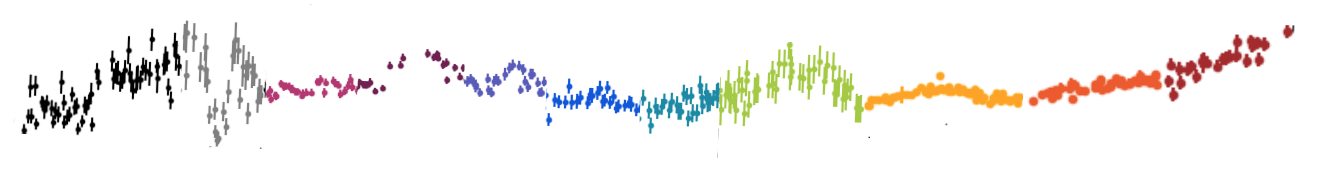
\includegraphics[width=\textwidth,height=1.4cm,keepaspectratio=false]{../../banner}\\[6pt]}
{\LARGE\bfseries\color{avaAbyss} A decade of LCO reverberation mapping key projects: telescope usage, data holdings and sources\par}
\vspace{6pt}
{\large\itshape\color{avaInkBlue} A metadata database of every image and spectrum, and its cross-match with the AVA AGN catalogue\par}
\noindent{\color{avaInkBlue}\rule{\textwidth}{1.5pt}}\\[12pt]
{\large\bfseries Juan V.\ Hern\'andez Santisteban}\\[2pt]
{\normalsize School of Physics and Astronomy, University of St Andrews, North Haugh, St Andrews, KY16~9SS, UK}\\[4pt]
{\small\color{avaInkBlue!70} AVA Internal Report \#\,2 $\cdot$ \reportDate}\\[22pt]
\begin{minipage}{0.92\textwidth}
\small\textbf{Abstract.} Since 2014 four Las Cumbres Observatory (LCO) key projects and their filler programmes have monitored nearby
active galactic nuclei for continuum and broad-line reverberation mapping. We built two SQLite databases holding
the metadata of every image (\nImages{} exposures, \firstImage{} to \lastImage) and every FLOYDS spectrum
(\nSpectra{} science spectra, \nArcs{} arcs and \nFlats{} lamp flats) taken by these programmes, without
downloading any image. The projects have been charged \hoursTotal{}~h (\msTotal~Ms) of telescope time, worth
\pounds\gbpTotal\,M (\$\usdTotal\,M) at current LCO prices. Every science spectrum is associated with its arcs,
lamp flats and the nearest flux standards, which come from \nStdProposals{} different proposals. Of the
\nAva{} AGN in the provisional AVA catalogue, \nAvaMatched{} have LCO data from these projects; \nNotInAvaFifty{}
further targets with at least 50 frames are not yet in the catalogue. The databases update daily.

\end{minipage}
\vfill
{\small\color{avaInkBlue!70} Keywords: galaxies: Seyfert --- techniques: photometric --- techniques: spectroscopic --- astronomical data bases: miscellaneous}
\end{titlepage}

\tableofcontents
\clearpage

\chapter*{Summary}
\addcontentsline{toc}{chapter}{Summary}
\begin{itemize}\setlength{\itemsep}{2pt}
\item \textbf{Telescope time.} \hoursTotal{}~h charged (\msTotal~Ms): \hoursOneM~h on the 1-m network and
  \hoursTwoM~h on the 2-m telescopes, i.e.\ \pounds\gbpTotal\,M (\$\usdTotal\,M) at today's list prices
  (\pounds\gbpTotalLow--\gbpTotalHigh\,M for 2-m prices between one and four times the 1-m rate).
  Shutter-open time is \expImagesMs~Ms of imaging and \expSpectraMs~Ms of FLOYDS science exposure.
\item \textbf{Images.} \nImages{} exposures of \nImageTargets{} targets in \nVisits{} visits:
  \nImagesSinistro{} Sinistro, \nImagesSpectral{} Spectral and \nImagesMuscat{} MuSCAT. BANZAI products
  (\nImagesNinetyOne) are used wherever they exist; \nImagesNinety{} early exposures only have the
  pre-BANZAI pipeline product.
\item \textbf{Spectra.} \nSpectra{} FLOYDS science spectra (\nSpecEpochs{} epochs, \nSpecTargets{} targets) from
  \firstSpectrum, each linked to its arcs and lamp flats (\fracArcBlock\,\% of best arcs from the same block) and
  to the nearest standards (\nStdFrames{} standard spectra of \nStdTargets{} stars).
\item \textbf{Image quality (1\,m).} Median airmass \medAirmass, median FWHM \medFwhm\,arcsec.
\item \textbf{Sources.} \nAvaMatched{} of the \nAva{} AVA AGN are observed; missing: \avaMissing.
  \nNotInAva{} other LCO target names have no AVA entry (\nNotInAvaFifty{} with $\geq 50$ frames); \nAvaReview{}
  matches need a check by eye.
\end{itemize}

\chapter{Introduction}\label{sec:intro}
Intensive broadband reverberation mapping needs dense, long and homogeneous light curves, which is what the LCO
key projects in Table~\ref{tab:proposals} have delivered since 2014: daily or sub-daily multi-band imaging on the
1-m network, complemented by 2-m imaging and FLOYDS spectroscopy. Reducing this data set systematically ---
re-extracting the FLOYDS spectra with the improved pipeline, building homogeneous light curves --- starts with
knowing exactly what was observed, when, with which instrument and calibrations, and under which conditions.

This report describes a metadata database of the whole data set built from the LCO archive API
(Chapter~\ref{sec:db}), the telescope time the projects have used and its value (Chapter~\ref{sec:usage}), the
photometric and spectroscopic holdings (Chapters~\ref{sec:phot} and \ref{sec:spec}), and the cross-match of the
observed targets with the provisional AVA catalogue of AGN (Chapter~\ref{sec:sources}).

\begin{table}[h]
\centering\small
\caption{The programmes included. KEY2014A-002 and KEY2018B-001 are led by other PIs; all others are led by the
author. Filler programmes (suffix f) use the same targets.}\label{tab:proposals}
\begin{tabular}{llll}
\toprule
Proposal & Role & Semesters & Title \\
\midrule
\inputtable{tables/tab_proposals.tex}
\bottomrule
\end{tabular}
\end{table}

\chapter{The database}\label{sec:db}
\section{Contents and construction}
The package \lcodb{} reads the LCO science archive (\texttt{archive-api.lco.global}) and the observation portal
(\texttt{observe.lco.global}) with the PI's API token and writes two SQLite databases:
\begin{itemize}\setlength{\itemsep}{1pt}
\item \texttt{photometry.sqlite}: Sinistro (camera prefixes \texttt{fa}, and \texttt{fl} for the early
  Sinistros), Spectral (\texttt{fs}) and MuSCAT (\texttt{ep}) images. Only reduced frames are kept: the BANZAI
  product (reduction level 91) and, where none exists, the earlier pipeline product (level 90; flag
  \texttt{is\_best}).
\item \texttt{spectra.sqlite}: FLOYDS raw frames (science, arcs, lamp flats) and BANZAI-FLOYDS products,
  plus the flux standards from any proposal (\S\ref{sec:standards}).
\end{itemize}
NRES, guide and acquisition cameras, catalogue files and experimental frames are excluded. Each frame keeps its
archive identifiers (so the file can be fetched later), target, coordinates, filter, exposure time, observing
block and request, the start time as ISO date, readable UTC (\texttt{date\_utc}) and MJD, and a set of header
keywords read from the archive's header service, which returns the full FITS header without the pixels. The
full header is also stored (compressed), so further keywords can be added as columns without new downloads.
An airmass is computed for every frame from the site, the footprint centre and the mid-exposure time; it agrees
with the header \texttt{AIRMASS} to 0.01.

\section{Header keywords across the decade}
A sample of headers from every year, camera and reduction level (2014--2026) showed that the keywords needed
for basic image quality are not homogeneous:
\begin{itemize}\setlength{\itemsep}{1pt}
\item \texttt{MJD-OBS} and \texttt{DATE-OBS} are missing from the headers served for frames before 2023; the
  database takes the time from the archive record instead, which is complete.
\item \texttt{TELID} only gives the class (\texttt{1m0a}); the individual telescope comes from the file name
  (\texttt{1m010}).
\item \texttt{SKYMAG} is the same in raw and reduced headers, i.e.\ it is a telemetry/scheduler value, and
  takes the placeholder 22.0 in many frames (\fracSkyPlaceholder\,\% of the 1-m images), which the quality view
  treats as missing.
\item \texttt{L1FWHM} uses $-99$ for failures in the old pipeline; \texttt{NAXIS1/2} is reliable in the
  reduced frames (4096 for BANZAI Sinistro, $4018\times3974$ for the old Sinistro products, 2009--2045 for
  binned Spectral, 2048 for MuSCAT).
\end{itemize}

\section{Daily update}
The first build crawled each proposal from its first semester in 30-day windows. The daily run re-reads the last
seven days of every active proposal, so late frames and new BANZAI versions are picked up (a changed checksum
triggers a new header download), fetches the missing headers, and rebuilds the calibration and standard
associations. New proposals in the PI profile are added automatically.

\chapter{Telescope time and its value}\label{sec:usage}
The observation portal records, for every proposal, semester and instrument class, the time allocated and the
time charged; charged time includes slews, acquisition and readout. Figure~\ref{fig:time} and
Table~\ref{tab:projects} summarise it, Fig.~\ref{fig:cost} gives the cumulative cost, and Appendix~\ref{sec:semesters} gives every semester.

\begin{figure}[h]
\centering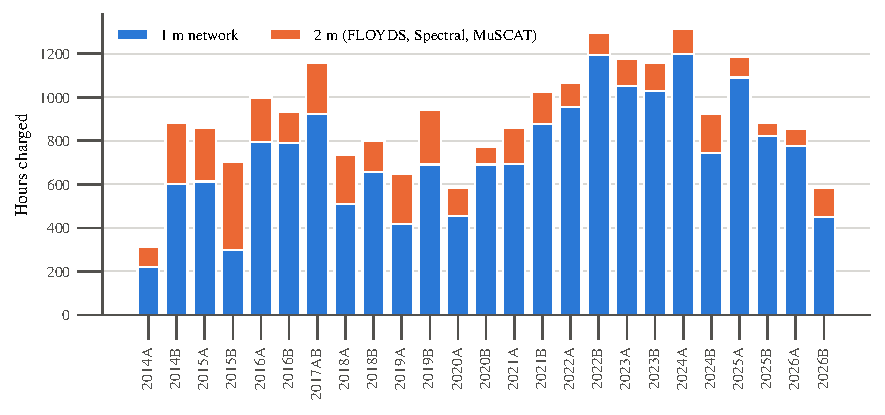
\includegraphics[width=\textwidth]{figures/fig_time_semester.pdf}
\caption{Telescope time charged per semester to the key projects, by telescope class. In 2014--2018 the 2-m time
is recorded as Spectral-camera time and includes the FLOYDS time.}\label{fig:time}
\end{figure}

\begin{table}[h]
\centering\small
\caption{Time charged and its value at current LCO prices, in pounds with dollars in parentheses
(\pounds\gbpOneM\,h$^{-1}$ = \$\usdOneM\,h$^{-1}$ on the 1-m network; 2-m time is not sold and is valued at \pounds\gbpTwoM\,h$^{-1}$ = \$\usdTwoM\,h$^{-1}$; \pounds\gbpPerUsd{} per \$). Images: reduced exposures in the
photometry database; spectra: FLOYDS science spectra.}\label{tab:projects}
\begin{tabular}{llrrrrrrr}
\toprule
Proposal & Semesters & 1-m (h) & 2-m (h) & Ms & \pounds\,M & (\$\,M) & Images & Spectra \\
\midrule
\inputtable{tables/tab_projects.tex}
\bottomrule
\end{tabular}
\end{table}

\begin{figure}[h]
\centering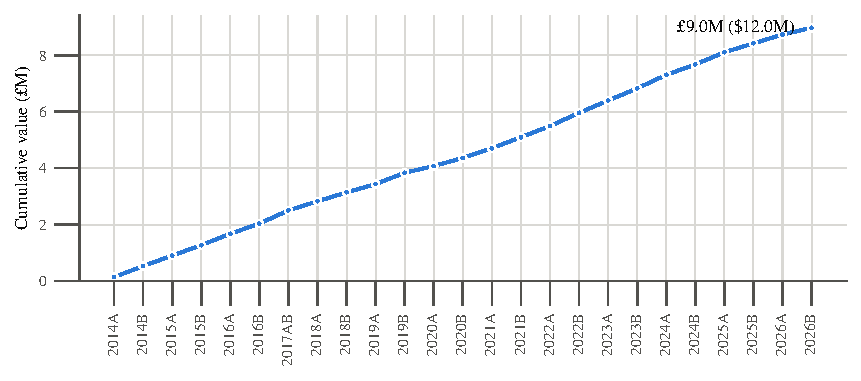
\includegraphics[width=\textwidth]{figures/fig_cost_cumulative.pdf}
\caption{Cumulative value of the time used, at current LCO prices (\pounds\gbpOneM\,h$^{-1}$ = \$\usdOneM\,h$^{-1}$ for
1-m time, an assumed \pounds\gbpTwoM\,h$^{-1}$ = \$\usdTwoM\,h$^{-1}$ for 2-m time).}\label{fig:cost}
\end{figure}

\paragraph{Value.} At the LCO price for 100\,h or more per year on the 1-m network (\pounds\gbpOneM\,h$^{-1}$,
\$\usdOneM\,h$^{-1}$) and an assumed \pounds\gbpTwoM\,h$^{-1}$ (\$\usdTwoM\,h$^{-1}$) for the 2-m telescopes, the
\hoursTotal~h used are worth \pounds\gbpTotal\,M (\$\usdTotal\,M). Pricing the 2-m time like the 1-m gives
\pounds\gbpTotalLow\,M (\$\usdTotalLow\,M), and scaling it by mirror area \pounds\gbpTotalHigh\,M (\$\usdTotalHigh\,M). Current prices are applied to all semesters.

\paragraph{Efficiency.} The open-shutter time is \expImagesMs~Ms for the images and \expSpectraMs~Ms for the FLOYDS
science spectra, against \msTotal~Ms charged. The imaging is about 70\,\% efficient on the 1-m network;
FLOYDS spends roughly two thirds of its charged time on acquisition, arcs, lamp flats and readout.

\chapter{Photometric data}\label{sec:phot}
The photometry database holds \nImages{} reduced exposures (\nImagesOneM{} on the 1-m telescopes) of
\nImageTargets{} targets in \nVisits{} visits (observing blocks), from \firstImage{} to \lastImage{}
(Fig.~\ref{fig:images}). The total open-shutter time is \expImagesH~h. Headers have been read for
\fracImagesHdr\,\% of them.

\begin{figure}[h]
\centering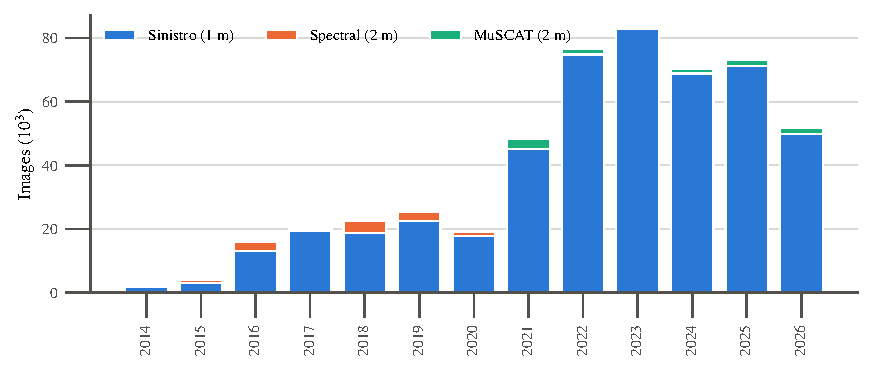
\includegraphics[width=\textwidth]{figures/fig_images_year.pdf}
\caption{Reduced images per year and camera.}\label{fig:images}
\end{figure}

\section{Basic quality of the 1-m images}
The view \texttt{image\_quality} gives, for each exposure, the quantities used for a first quality cut:
filter, object, exposure time, date and MJD, airmass, image size, site, sky brightness, telescope and pixel
scale, plus the BANZAI FWHM. Their distributions for the 1-m images are in Fig.~\ref{fig:quality}: the median
airmass is \medAirmass{} and the median FWHM \medFwhm\,arcsec.

\begin{figure}[h]
\centering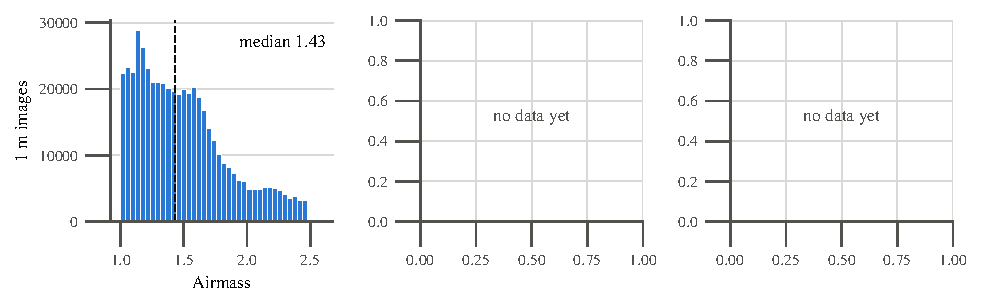
\includegraphics[width=\textwidth]{figures/fig_quality_1m.pdf}
\caption{Airmass, BANZAI image FWHM and header sky brightness of the 1-m images (placeholder sky values of 22.0
excluded). Dashed: median.}\label{fig:quality}
\end{figure}

\chapter{Spectroscopic data}\label{sec:spec}
The spectra database holds \nSpectra{} FLOYDS science spectra in \nSpecEpochs{} epochs of \nSpecTargets{}
targets since \firstSpectrum{} (Fig.~\ref{fig:spectra}), \expSpectraH~h of exposure, together with \nArcs{} arcs
and \nFlats{} lamp flats. \fracSixArcsec\,\% of the science spectra were taken with the 6-arcsec slit.

\begin{figure}[h]
\centering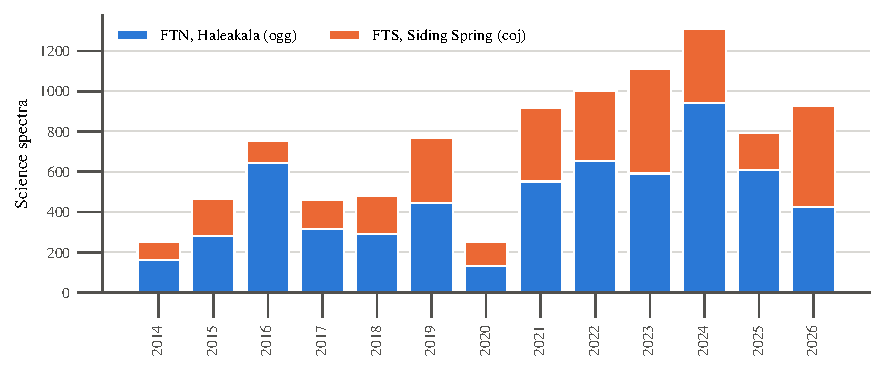
\includegraphics[width=\textwidth]{figures/fig_spectra_year.pdf}
\caption{FLOYDS science spectra per year and telescope.}\label{fig:spectra}
\end{figure}

\section{Arcs and lamp flats}
Each raw spectrum (science and standards) is linked to the arcs and lamp flats on the same spectrograph within
seven days, ranked by: same observing block, then same slit width, then time; the best three of each type are
kept (\texttt{calib\_match}). The best arc comes from the same block for \fracArcBlock\,\% of the spectra and the
best lamp flat for \fracFlatBlock\,\%; \nNoArc{} spectra have no arc within seven days.

\section{Flux standards}\label{sec:standards}
The key projects took few standards of their own. The standards were therefore collected by name from any
proposal: observatory calibration programmes (\texttt{COJ\_calib}, \texttt{OGG\_calib}, \texttt{FLOYDS standards},
engineering) and other key projects, \nStdFrames{} spectra of \nStdTargets{} stars from \nStdProposals{}
proposals (Table~\ref{tab:standards}). For each science spectrum the five nearest standards of each slit width
on the same spectrograph are kept, with a standard in the same block ranked first (\texttt{std\_match}). The
nearest standard is a median of \medStdDt~h away (Fig.~\ref{fig:stddt}); a standard with the same slit width
exists for \fracSameSlit\,\% of the spectra, a median of \medStdDtSame~d away. Most observatory standards are
taken with the 2-arcsec slit while the science uses 6 arcsec, which is the main limitation for the flux calibration.

The standard used for each science spectrum (view \texttt{spectrum\_standards}) is chosen in this order: the
nearest standard taken with the same slit width; failing that, the nearest standard taken with the 2-arcsec slit;
failing that, the nearest standard with any slit (a standard in the same block always wins over time). The three
cases apply to \nPickSame, \nPickTwo{} and \nPickAny{} science spectra, and \nPickNone{} have no standard on the same
spectrograph within 30~d. Spectra whose headers are not yet in the database have no known slit width and fall in
the second or third case.

\begin{figure}[h]
\centering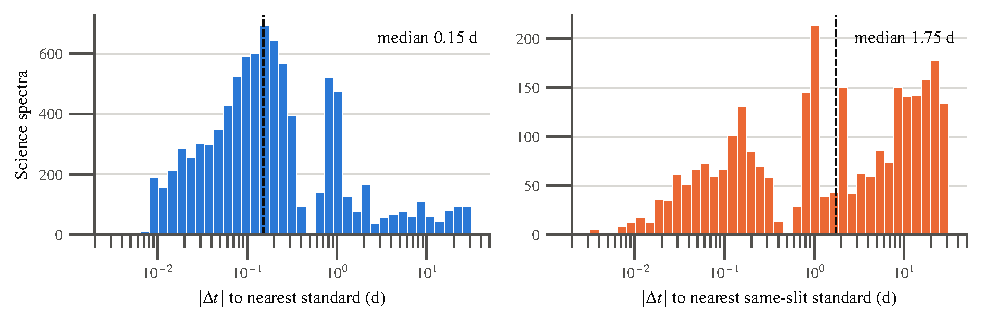
\includegraphics[width=\textwidth]{figures/fig_std_dt.pdf}
\caption{Time to the nearest standard (left) and to the nearest standard with the same slit width (right).}\label{fig:stddt}
\end{figure}

\begin{small}
\begin{longtable}{lrlrrp{5.2cm}}
\caption{Flux standards in the spectra database: number of spectra, date range, slit widths, number of science
spectra for which it is the selected standard, and the proposals they come from.}\label{tab:standards}\\
\toprule
Star & N & Dates & Slits & Best for & Proposals \\
\midrule\endfirsthead
\toprule
Star & N & Dates & Slits & Best for & Proposals \\
\midrule\endhead
\inputtable{tables/tab_standards.tex}
\bottomrule
\end{longtable}
\end{small}

\chapter{Sources and the AVA catalogue}\label{sec:sources}
\section{Cross-match}
The LCO target names are not uniform (\texttt{Fairall9} and \texttt{Fairall 9}; \texttt{MCG\_08-11-011},
\texttt{MCG 8-11-11} and \texttt{MCG\_08-11-11}; \texttt{Mrk 1044} and \texttt{Mrk1044}). Each LCO name is
therefore given a position --- the median requested coordinates from the headers (\texttt{CAT-RA},
\texttt{CAT-DEC}), or the median footprint centre when no header is available --- and matched to the AVA
catalogue within 30\,arcsec (3\,arcmin for footprint positions) or by normalised name. Of the \nAva{} AVA
sources, \nAvaMatched{} are observed by the key projects (Fig.~\ref{fig:sky}); \avaMissing{} are not. \nAvaReview{}
matches by name have discrepant positions and are flagged for inspection.

The AVA table is the master target list. Every frame in both databases carries the AVA identifier of its target
(\texttt{frames.ava\_id} and \texttt{ava\_data\_id}; the name-to-identifier links are in table
\texttt{target\_link}), refreshed at every daily update, so any image or spectrum can be selected by AGN regardless
of how its target was named at the telescope. Manual decisions (for example, the offset fields of NGC~4395) go in
\texttt{AVA/ava\_link\_overrides.csv} and take precedence over the automatic match. The AVA table itself is also
kept as an SQLite database, \texttt{AVA/ava.sqlite} (the original table verbatim in \texttt{agn}, the recomputed LCO
statistics in \texttt{agn\_lco}, and the links in \texttt{lco\_targets}), with two CSV copies: \texttt{ava.csv}
(all columns, with header) and \texttt{ava\_nohead.csv} (the original columns, without header, byte-identical to
the master rows).

The LCO columns of the AVA table are refreshed from the databases (Table~\ref{tab:ava}) in a new file
\texttt{AVA/ava\_lco\_updated.csv}, which keeps the previous values (\texttt{*\_prev}) and leaves the Swift and
Liverpool Telescope columns untouched. The counts include only the key projects listed in
Table~\ref{tab:proposals}; the earlier AVA values for some sources also included other programmes (e.g.\ AGN
STORM~2 for Mrk~817), so a lower number is not a loss of data. Cadences are medians of the intervals between visits.

\begin{figure}[h]
\centering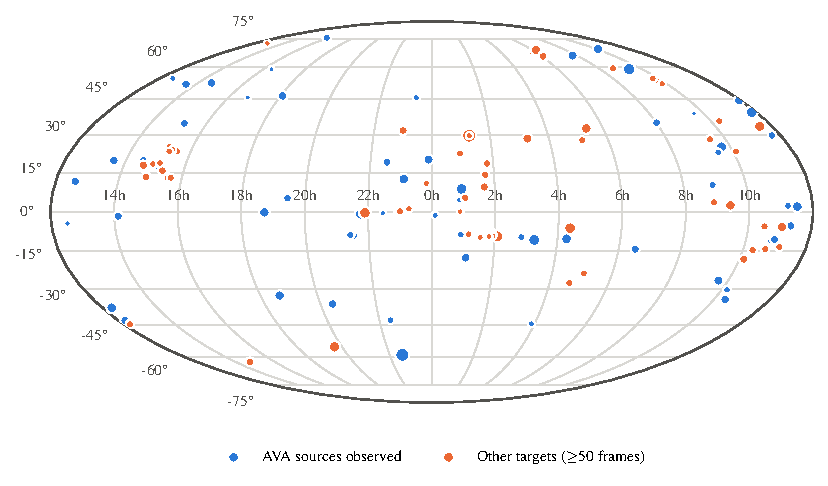
\includegraphics[width=0.9\textwidth]{figures/fig_sky.pdf}
\caption{Sky positions of the AVA sources observed by the key projects and of other LCO targets with at least
50 frames; symbol size grows with the number of frames.}\label{fig:sky}
\end{figure}

\begin{small}
\setlength{\tabcolsep}{4pt}
\begin{longtable}{lrrrlrrlp{2.4cm}}
\caption{LCO holdings of the AVA sources: reduced images, visits, median imaging cadence (d), imaging dates,
FLOYDS epochs, median spectroscopic cadence (d), FLOYDS dates and the key projects that observed it
(e.g.\ 23Bf = KEY2023B-001f).}\label{tab:ava}\\
\toprule
Source & Images & Visits & Cad. & Imaging & Ep. & Cad. & FLOYDS & KP \\
\midrule\endfirsthead
\toprule
Source & Images & Visits & Cad. & Imaging & Ep. & Cad. & FLOYDS & KP \\
\midrule\endhead
\inputtable{tables/tab_ava.tex}
\bottomrule
\end{longtable}
\end{small}

\section{Properties of the sample}
Table~\ref{tab:properties} lists the AVA sources with their redshift, Galactic reddening, mean $g$ magnitude,
luminosity, Eddington ratio and black-hole mass from the AVA catalogue, and the imaging and FLOYDS cadences
measured from the database.

\begin{small}
\setlength{\tabcolsep}{3.5pt}
\begin{longtable}{lccccccccrr}
\caption{The AVA sample, ordered by right ascension. $z$, E($B-V$), $g$ (mean LCO magnitude), $\log L$,
$L/L_{\rm Edd}$ and $\log M_{\rm BH}$ are from the AVA catalogue; the cadences are the median intervals between
LCO imaging visits and between FLOYDS epochs in the key projects (Table~\ref{tab:proposals}).}\label{tab:properties}\\
\toprule
Name & RA & Dec & $z$ & E($B-V$) & $g$ & $\log L$ & $L/L_{\rm Edd}$ & $\log M_{\rm BH}$ & LCO cadence & FLOYDS cadence \\
 & hh mm ss.s & $\pm$dd mm ss & & & mag & erg\,s$^{-1}$ & & M$_\odot$ & day & day \\
\midrule\endfirsthead
\multicolumn{11}{l}{\small\itshape Table \ref{tab:properties} -- continued}\\
\toprule
Name & RA & Dec & $z$ & E($B-V$) & $g$ & $\log L$ & $L/L_{\rm Edd}$ & $\log M_{\rm BH}$ & LCO cadence & FLOYDS cadence \\
 & hh mm ss.s & $\pm$dd mm ss & & & mag & erg\,s$^{-1}$ & & M$_\odot$ & day & day \\
\midrule\endhead
\bottomrule\endfoot
\inputtable{tables/tab_properties.tex}
\end{longtable}
\end{small}

\section{Targets not in the catalogue}
\nNotInAva{} LCO target names have no AVA counterpart; \nNotInAvaFifty{} of them have at least 50 frames.
They include AGN that should be added (Table~\ref{tab:new}) as well as photometric comparison fields and
short test observations.

\begin{small}
\begin{longtable}{lrrrr}
\caption{LCO targets without an AVA counterpart, by number of frames (first 40).}\label{tab:new}\\
\toprule
LCO name & RA (deg) & Dec (deg) & Images & Spectra \\
\midrule\endfirsthead
\toprule
LCO name & RA (deg) & Dec (deg) & Images & Spectra \\
\midrule\endhead
\inputtable{tables/tab_new.tex}
\bottomrule
\end{longtable}
\end{small}

\chapter{Software and maintenance}\label{sec:software}
\begin{itemize}\setlength{\itemsep}{1pt}
\item \texttt{lco\_archive\_db/} -- the \lcodb{} package: \texttt{config.yaml} (proposals, instruments, levels,
  standards, rates), \texttt{lcodb daily} for the update, \texttt{lcodb status} for a summary; offline tests in
  \texttt{tests/}.
\item \texttt{lco\_archive\_db/tools/header\_audit.py} -- header keyword coverage across years and cameras.
\item \texttt{lco\_archive\_db/tools/cost\_estimate.py} -- hours and value per project and semester.
\item \texttt{lco\_archive\_db/tools/ava\_crossmatch.py} -- AVA cross-match and refreshed table.
\item \texttt{lco\_report/scripts/make\_report.py} -- all numbers, tables and figures of this report.
\end{itemize}
To refresh the report: \texttt{lcodb daily}; \texttt{python3 tools/ava\_crossmatch.py --ava ../AVA/ava\_testdb\_whead.csv
--outdir ../AVA}; \texttt{python3 scripts/make\_report.py}; \texttt{latexmk -pdf lco\_usage\_report.tex}.


\chapter*{Acknowledgements}
\addcontentsline{toc}{chapter}{Acknowledgements and data availability}
Based on observations obtained with the Las Cumbres Observatory global telescope network.
The metadata were read from the LCO science archive and observation portal APIs; no image was
downloaded to build the databases.

\appendix
\chapter{Time per semester}\label{sec:semesters}
\begin{small}
\begin{longtable}{lllrrrrrr}
\caption{Time charged per proposal and semester: instruments used, hours on the 1-m and 2-m telescopes,
allocation, fraction used and value in thousands of pounds (dollars).}\\
\toprule
Proposal & Sem. & Instruments & 1-m (h) & 2-m (h) & Alloc. (h) & Used (\%) & k\pounds & (k\$) \\
\midrule\endfirsthead
\toprule
Proposal & Sem. & Instruments & 1-m (h) & 2-m (h) & Alloc. (h) & Used (\%) & k\pounds & (k\$) \\
\midrule\endhead
\inputtable{tables/tab_semesters.tex}
\bottomrule
\end{longtable}
\end{small}

\chapter{Database tables}\label{sec:schema}
\paragraph{\texttt{frames}} (both databases) one row per archive frame: identifiers (\texttt{id}, \texttt{basename},
\texttt{filename}, \texttt{exp\_key}, \texttt{raw\_id}), \texttt{proposal\_id}, \texttt{instrument\_id},
\texttt{site\_id}, \texttt{telescope\_id}, \texttt{tel\_key}, \texttt{date\_obs}, \texttt{date\_utc}, \texttt{day\_obs},
\texttt{mjd\_obs}, \texttt{object}, \texttt{ra}, \texttt{dec}, \texttt{filter}, \texttt{exptime}, \texttt{obstype},
\texttt{rlevel}, \texttt{block\_id}, \texttt{request\_id}, \texttt{is\_best}, \texttt{is\_standard},
\texttt{airmass\_calc}; header columns \texttt{airmass}, \texttt{agfwhm}, \texttt{l1fwhm}, \texttt{l1zp},
\texttt{l1zperr}, \texttt{l1mean}, \texttt{l1sigma}, \texttt{skymag}, \texttt{wmsskybr}, \texttt{wmscloud},
\texttt{wmshumid}, \texttt{moondist}, \texttt{moonfrac}, \texttt{moonalt}, \texttt{sunalt}, \texttt{altitude},
\texttt{azimuth}, \texttt{cat\_ra}, \texttt{cat\_dec}, \texttt{srctype}, \texttt{moltype}, \texttt{groupid},
\texttt{userid}, \texttt{aperwid}, \texttt{apertype}, \texttt{rotmode}, \texttt{rotskypa}, \texttt{confmode},
\texttt{ccdsum}, \texttt{pixscale}, \texttt{naxis1}, \texttt{naxis2}, \texttt{gain}, \texttt{rdnoise},
\texttt{saturate}, \texttt{utstop}.
\paragraph{\texttt{headers}} the full FITS header of each frame, compressed JSON.
\paragraph{Views} \texttt{images} and \texttt{image\_quality} (photometry); \texttt{exposures} and
\texttt{spectrum\_calibs} (spectra); \texttt{targets} (both).
\paragraph{\texttt{std\_match}, \texttt{calib\_match}} (spectra) the standard and arc/flat associations.
\paragraph{\texttt{state.sqlite}} \texttt{sync\_state} (per proposal), \texttt{runs} (log),
\texttt{unknown\_instruments}.


\end{document}
